%!TEX root = thesis.tex
%% %% ***************** Appendices *****************

\clearpage


\thesisappendix

\section{Final pipeline structure}\label{sec:app-final-pipeline-structure}
{
    \scriptsize
    Final pipeline includes message and rawmessage branches, their pure, preprocessed and feature hashing combinations,
    two algorithm comparison blocks, and a three final test branches using fresh data for for model scoring.
}
\begin{figure}[htb]
    \centering
    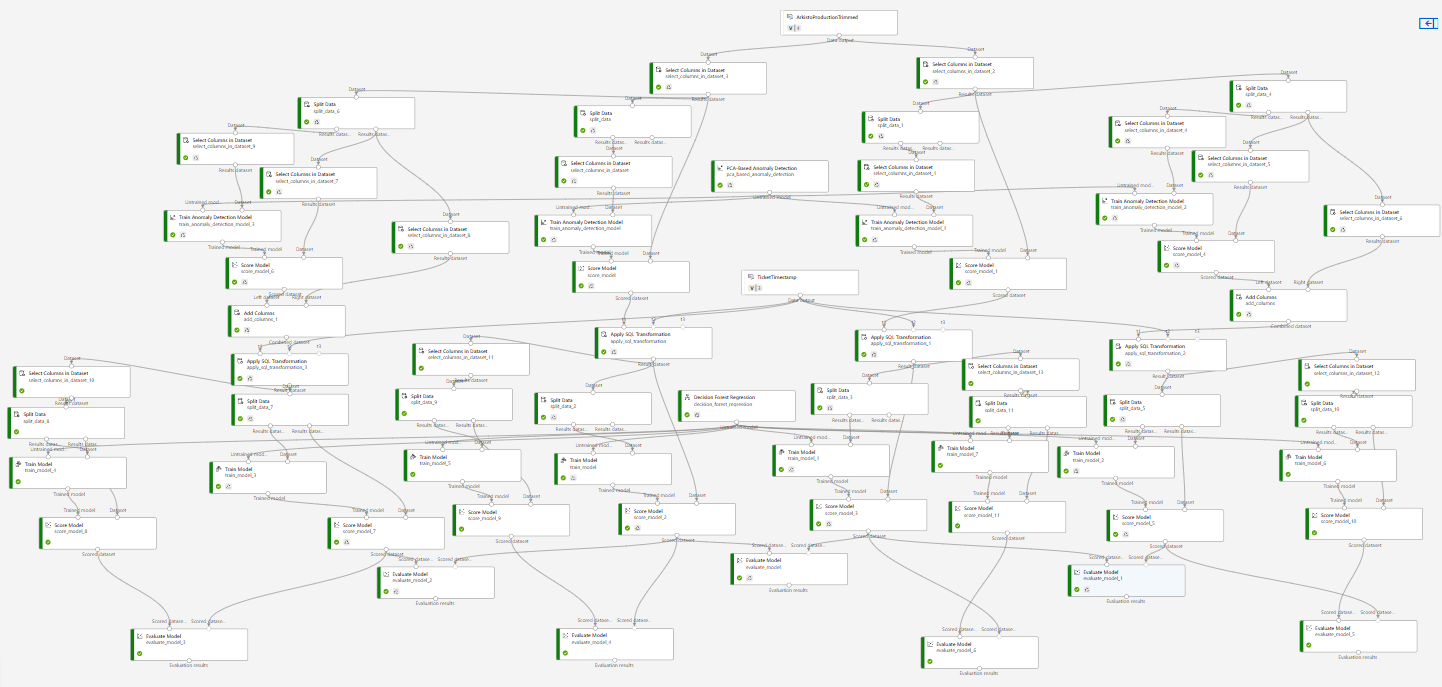
\includegraphics[width=202mm,height=\textwidth,angle=90]{./appendices/pipeline-draft}
\end{figure}

\clearpage

%% ************************************************************************************************************

\section{RPA log data example}\label{sec:app-log-data-input}

RPA log data in raw format after anonymizing and exporting to local environment.
Here are four lines of log events with different log levels,
first line being a header row.
First example has been reduced in size with \verb-[...]--marking.
Data is in CSV-format,
with each column separated by comma.
The rawmessage is injected inside CSV
in JSON-format.

This data was fetched from the SQL-database
with the following SQL-script:
\verb=SELECT OrganizationUnitId,TenantId,TimeStamp,Level,=

\verb=ProcessName,JobKey,RobotName,Message,RawMessage,=

\verb=MachineId FROM [dbo].[logs]=

\begin{Verbatim}[fontsize=\tiny]
"OrganizationUnitId","TenantId","TimeStamp","Level","ProcessName","JobKey","RobotName","Message","RawMessage","MachineId"
"5","5","1/2/2020 12:55:24 PM","4","rpa-bank-020-lainahakemuksien-tietojen-siirto_Samlink Production",
    "b03cfd05-1807-45e7-b962-c9d95e49a3fc","RPA-RPP-4","System.IO.IOException: The process cannot access the file
    'W:\RPA\BANK\020 lainahakemuksien tietojen siirto\prod\Config.xlsx' because it is being used by another process.
    at System.IO.__Error.WinIOError(Int32 errorCode, String maybeFullPath)
    at System.IO.FileStream.Init(String path, FileMode mode, FileAccess access, Int32 rights, Boolean useRights,
        FileShare share, Int32 bufferSize, FileOptions options, SECURITY_ATTRIBUTES secAttrs, String msgPath, Boolean
        bFromProxy, Boolean useLongPath, Boolean checkHost)
    at System.IO.FileStream..ctor(String path, FileMode mode, FileAccess access, FileShare share, Int32 bufferSize,
        FileOptions options, String msgPath, Boolean bFromProxy)
    at System.IO.FileStream..ctor(String path, FileMode mode, FileAccess access, FileShare share, Int32 bufferSize,
        Boolean useAsync)
        [...]
    at System.Activities.Runtime.ActivityExecutor.ExecuteActivityWorkItem.ExecuteBody(ActivityExecutor executor,
        BookmarkManager bookmarkManager, Location resultLocation)","{
    "message": "System.IO.IOException: The process cannot access the file 'W:\\RPA\\BANK\\020 lainahakemuksien tietojen
        siirto\\prod\\Config.xlsx' because it is being used by another process.\r\n   at System.IO.__Error.WinIOError
        (Int32 errorCode, String maybeFullPath)\r\n   at System.IO.FileStream.Init(String path, FileMode mode,
        FileAccess access, Int32 rights, Boolean useRights, FileShare share, Int32 bufferSize, FileOptions options,
        SECURITY_ATTRIBUTES secAttrs, String msgPath, Boolean bFromProxy, Boolean useLongPath, Boolean checkHost)\r\n
        at System.IO.FileStream..ctor(String path, FileMode mode, FileAccess access, FileShare share, Int32 bufferSize,
        FileOptions options, String msgPath, Boolean bFromProxy)\r\n   at System.IO.FileStream..ctor(String path,
        FileMode mode, FileAccess access, FileShare share, Int32 bufferSize, Boolean useAsync) [...]   at
        System.Activities.Runtime.ActivityExecutor.ExecuteActivityWorkItem.ExecuteBody(ActivityExecutor executor,
        BookmarkManager bookmarkManager, Location resultLocation)",
    "level": "Error",
    "logType": "User",
    "timeStamp": "2020-01-02T14:55:24.6280687+02:00",
    "fingerprint": "5ebb011b-fb3d-402a-8024-79a21e6629c9",
    "windowsIdentity": "LOCAL\\WinID",
    "machineName": "T4690A3018",
    "processName": "rpa-bank-020-lainahakemuksien-tietojen-siirto_Samlink Production",
    "processVersion": "1.0.7244.25507",
    "jobId": "b03cfd05-1807-45e7-b962-c9d95e49a3fc",
    "robotName": "RPA-RPP-4",
    "machineId": 28,
    "fileName": "GlobalHandler"
}","28"
"5","5","1/2/2020 12:55:24 PM","0","rpa-bank-020-lainahakemuksien-tietojen-siirto_Samlink Production",
    "b03cfd05-1807-45e7-b962-c9d95e49a3fc","RPA-RPP-4","Log Error Executing","{
    "message": "Log Error Executing",
    "level": "Verbose",
    "logType": "Default",
    "timeStamp": "2020-01-02T14:55:24.6280687+02:00",
    "fingerprint": "3c68aacf-dd4c-4ad4-8045-043e72b35bb7",
    "windowsIdentity": "LOCAL\\WinID",
    "machineName": "T4690A3018",
    "processName": "rpa-bank-020-lainahakemuksien-tietojen-siirto_Samlink Production",
    "processVersion": "1.0.7244.25507",
    "jobId": "b03cfd05-1807-45e7-b962-c9d95e49a3fc",
    "robotName": "RPA-RPP-4",
    "machineId": 28,
    "fileName": "GlobalHandler",
    "activityInfo": {
        "Activity": "UiPath.Core.Activities.LogMessage",
        "DisplayName": "Log Error",
        "State": "Executing",
        "Variables": {
            "answer": "",
            "retry": "0",
            "HetuFound": "False",
            "FilteredException": ""
        },
        "Arguments": {
            "Message": "System.IO.IOException: The process cannot access the file 'W:\\RPA\\BANK\\020 lainahakemuksien
                tietojen siirto\\prod\\Config.xlsx' because it is being used by another process.\r\n   at System.IO.
                __Error.WinIOError(Int32 errorCode, String maybeFullPath)\r\n   at System.IO.FileStream.Init(String
                path, FileMode mode, FileAccess access, Int32 rights, Boolean useRights, FileShare share, Int32
                bufferSize, FileOptions options, SECURITY_ATTRIBUTES secAttrs, String msgPath, Boolean bFromProxy,
                Boolean useLongPath, Boolean checkHost)\r\n   at System.IO.FileStream..ctor(String path, FileMode mode,
                FileAccess access, FileShare share, Int32 bufferSize, FileOptions options, String msgPath, Boolean
                bFromProxy)\r\n   at System.IO.FileStream..ctor(String path, FileMode mode, FileAccess access, FileShare
                share, Int32 bufferSize, Boolean useAsync)\r\n   at MS.Internal.IO.Zip.ZipArchive.OpenOnFile(String
                path, FileMode mode, FileAccess access, FileShare share, Boolean streaming)\r\n   at System.IO.
                Packaging.ZipPackage..ctor(String path, FileMode mode, FileAccess access, FileShare share, Boolean
                streaming)\r\n   at System.IO.Packaging.Package.Open(String path, FileMode packageMode, FileAccess
                packageAccess, FileShare packageShare, Boolean streaming)\r\n   at DocumentFormat.OpenXml.Packaging.
                OpenXmlPackage.OpenCore(String path, Boolean readWriteMode)\r\n   at DocumentFormat.OpenXml.Packaging.
                SpreadsheetDocument.Open(String path, Boolean isEditable, OpenSettings openSettings)\r\n   at ClosedXML.
                Excel.XLWorkbook.LoadSheets(String fileName) in C:\\Projects\\ClosedXML\\ClosedXML\\Excel\\XLWorkbook
                _Load.cs:line 44\r\n   at UiPath.Excel.WorkbookFile..ctor(String workbookPath, String password, Boolean
                createNew)\r\n   at UiPath.Excel.Activities.WorkbookActivity`1.ConstructWorkbook(String path, String
                password, Boolean createNew)\r\n   at UiPath.Excel.Activities.WorkbookActivity`1.BeginExecute(
                AsyncCodeActivityContext context, AsyncCallback callback, Object state)\r\n   at System.Activities.
                AsyncCodeActivity.InternalExecute(ActivityInstance instance, ActivityExecutor executor, BookmarkManager
                bookmarkManager)\r\n   at System.Activities.ActivityInstance.Execute(ActivityExecutor executor,
                BookmarkManager bookmarkManager)\r\n   at System.Activities.Runtime.ActivityExecutor.
                ExecuteActivityWorkItem.ExecuteBody(ActivityExecutor executor, BookmarkManager bookmarkManager, Location
                resultLocation)"
        }
    }
}","28"
"5","5","8/11/2021 10:14:26 PM","3","rpa-bank-011-ott-valmistelu-4503","5186baa6-6f2d-4cc0-8001-a78f518579fb",
    "RPA-RPP-1-4503","Screenshot saved at: G:\Robotiikka\011 OTT Valmis\prod\Screensh\ExceptionScreenshot_.011426.png","{
    "message": "Screenshot saved at: G:\\Robotiikka\\011 OTT Valmis\\prod\\Screensh\\ExceptionScreenshot_.011426.png",
    "level": "Warning",
    "logType": "User",
    "timeStamp": "2021-08-12T01:14:26.3516259+03:00",
    "fingerprint": "3ced557c-7a73-4e0c-bd73-1759fbbd8cca",
    "windowsIdentity": "LOCAL\\WinID",
    "machineName": "T4690K3336",
    "processName": "rpa-bank-011-ott-valmistelu-4503",
    "processVersion": "1.6.7769.24916",
    "jobId": "5186baa6-6f2d-4cc0-8001-a78f518579fb",
    "robotName": "RPA-RPP-1-4503",
    "machineId": 38,
    "organizationUnitId": 5,
    "fileName": "TakeScreenshot",
    "logF_BusinessProcessName": "rpa-bank-011-OTT-valmistelu"
}","38"
"5","5","8/11/2021 9:46:52 PM","2","rpa-bank-011-ott-valmistelu-4260","66d75a97-9f08-401c-8e27-b1d23463a44f",
    "RPA-RPP-2-4260","Kaikkien tilien saldo tälle hetulle nyt: 1.05","{
    "message": "Kaikkien tilien saldo tälle hetulle nyt: 1.05",
    "level": "Information",
    "logType": "User",
    "timeStamp": "2021-08-12T00:46:52.328433+03:00",
    "fingerprint": "5b4c9287-eb8d-4fb0-9e21-015eee3b3adb",
    "windowsIdentity": "LOCAL\\WinID",
    "machineName": "T4690A3016",
    "processName": "rpa-bank-011-ott-valmistelu-4260",
    "processVersion": "1.6.7769.24916",
    "jobId": "66d75a97-9f08-401c-8e27-b1d23463a44f",
    "robotName": "RPA-RPP-2-4260",
    "machineId": 11,
    "organizationUnitId": 5,
    "fileName": "TilienSaldot",
    "logF_BusinessProcessName": "rpa-bank-011-OTT-valmistelu"
}","11"

\end{Verbatim}

\clearpage

%% ************************************************************************************************************


\section{Anonymization script}\label{sec:app-anonymization-script}

Next here is the PowerShell script used
to anonymize the RPA log data.
During data fetching with SQL,
special string tokens were added at the beginning and the end of each row
for anonymizing script to separate each row.
This was because of the rawmessage-field
which included line breaks
and thus span of one log entry could be over dozens of rows in CSV file.

As data size was multiple gigabytes,
it was impossible to read it to memory in one go.
Instead,
stream reading was applied.
Script reads one log entry to the memory,
makes necessary processing and anonymization,
and outputs the entry in one line to output file
before reading the next row.

\begin{Verbatim}[fontsize=\tiny]

# UltimateAnonymizer.ps
# This script converts product data to pure CSV and anonymizes it on the go

$prodLevel = "tuotanto"

# Input file path
$path = "C:\dippa\tuotanto\tuotanto_arkisto_$prodLevel.csv"
$errorLogPath = "C:\dippa\tuotanto\ultimate_error.log"
$logpath = "C:\dippa\tuotanto\ultimate_run.log"

Out-File -Encoding utf8 -FilePath $logpath
Add-Content $logpath "$(Get-Date): Starting powershell script"

Out-File -Encoding utf8 -FilePath $errorLogPath

# Output file path
# Important: specify a *full* path
$outFileStream = [System.IO.StreamWriter] "C:\dippa\tuotanto\tuotanto_arkisto_$prodLevel`_final.csv"

$lineCounter = 0
$json = ''

$outFileStream.WriteLine('"organizationUnitId","level","logType","timeStamp","fingerprint","machineName",
    "processName","jobId","robotName","machineId","message","rawmessage"')

$SSNregex = "(?<![a-zA-Z0-9])[\d]{6}[-a+]?[\d]{3}[\w]{1}(?:0{0}|0{3})(?![a-zA-Z0-9])"
$EMAILregex = "[^\`"\s]+@[\.\w-]*[\w]"
$IBANregex = "(?:(?<![a-zA-Z0-9])|(?<=\\\D))(?:FI|fi)(?: ?\d){16}(?![a-zA-Z0-9])"
$BBANDASHregex = "(?<![a-zA-Z0-9])[\d]{6}-[\d]{2,8}(?![a-zA-Z0-9])"
$PHONEINTregex = "(?<![a-zA-Z0-9])\+358(?: ?\d){8,10}(?![a-zA-Z0-9])"
$PHONEregex = "(?<![a-zA-Z0-9-])[0][\d]{2,3}[ -]?(?: ?\d){6,8}(?![a-zA-Z0-9-])"
$BUSINESSregex = "(?<![a-zA-Z0-9])[\d]{7}-[\d]{1}(?![a-zA-Z0-9])"
$BUSINESSINTregex = "(?<![a-zA-Z0-9])[a-zA-Z]{2}[\d]{8}(?![a-zA-Z0-9])"
$BUSINESSINTZEROregex = "(?<![a-zA-Z0-9])[0]{2}[\d]{8}(?![a-zA-Z0-9])"
$CCregex = "(?<![a-zA-Z0-9-.])[\d]{1}(?: ?\d){14,15}(?![a-zA-Z0-9-])"
$WINIDregex = "(?<![a-zA-Z0-9])[a-zA-Z]{1,2}[\d]{6}(?![a-zA-Z0-9])"
$ADDRCOMregex = "[^\s""',.]* ?(katu|tie|kuja|polku|kaari|linja|raitti|rinne|penger|ranta|väylä|taival|tanhua|portti
    |veräjä|laita|reuna|syrjä|aukio|tori|laituri|tunneli) [\d]{1,3}( ?[a-zA-Z.]{1,4} ?[\d]{0,3})?(?!\w)"
$ADDRZIPregex = "(?<=\s)[\S]* [\d]{1,3}( ?[a-zA-Z.]{1,4} ?[\d]{0,3})?(\s|,\s)[\d]{5}(?!\w)"
$BankIDregex = "(?<![a-zA-Z0-9-])[\d]{8}(?![a-zA-Z0-9-])"
$BBANnoDASHregex = "(?<![a-zA-Z0-9])[\d]{14}(?![a-zA-Z0-9])"
$BUSINESSArtificialregex = "(?<![a-zA-Z0-9])[89]{1}[\d]{9}(?![a-zA-Z0-9])"

function Hide-Sensitive {
    param (
        [Parameter(Mandatory, ValueFromPipeline)]
        [string]$sensitiveLine
    )
    # OBS! If number is replaced with letters,
    # it is possible we break JSON key-value pair where value is (was) number.
    # This is why possibly only number containing strings are replaced to numbers
    $sensitiveLine -replace $SSNregex ,"10105051470101" `
            -replace $EMAILregex ,"EmailAddress0101" `
            -replace $IBANregex ,"1010IBANnumber0101" `
            -replace $BBANDASHregex ,"1010BBANnumber0101" `
            -replace $BBANnoDASHregex ,"101088420101" `
            -replace $PHONEINTregex ,"1010PhoneNumberInt0101" `
            -replace $PHONEregex ,"1010980230101" `
            -replace $BUSINESSregex ,"1010BusinessID0101" `
            -replace $BUSINESSINTregex ,"101086512350101" `
            -replace $BUSINESSINTZEROregex ,"1010865123500101" `
            -replace $BUSINESSArtificialregex ,"101086512354970101" `
            -replace $CCregex ,"1010664900101" `
            -replace $BankIDregex ,"10108426100101" `
            -replace $WINIDregex ,"1010WinID0101" `
            -replace $ADDRCOMregex ,"1010AddressCommon0101" `
            -replace $ADDRZIPregex ,"1010AddressZip0101" `
}

function Write-Json {
    param (
        [Parameter(Mandatory, ValueFromPipeline)]
        [string]$json
    )
    try {
        # From each message/rawmessage field, first filter out all line endings, then remove unnecessary special characters,
        # excess whitespaces, and finally anonymize sensitive information
        ($json | ConvertFrom-Json).SyncRoot |
        Select-Object organizationUnitId,level,logType,timeStamp,fingerprint,machineName,processName,jobId,robotName,machineId,
        @{l='message';e={$_.message -replace '(\r|\n|`r|`n)', '' -replace '[^\p{L}\p{Nd} .,\-_\/(){}\[\]:+]',
            '' -replace '\s+', ' ' | Hide-Sensitive}},
        @{l='rawmessage';e={[System.Text.RegularExpressions.Regex]::Unescape($json) -replace '(\r|\n|`r|`n)',
            '' -replace '[^\p{L}\p{Nd} .,\-_\/(){}\[\]:+]', '' -replace '\s+', ' ' | Hide-Sensitive}} |
        ConvertTo-Csv -NoTypeInformation |
        Select-Object -Skip 1 |
        Foreach-Object { $outFileStream.WriteLine($_) }
    }
    catch {
        Add-Content $errorLogPath "$(Get-Date): Found some errors with data during writing JSON to CSV:"
        Add-Content $errorLogPath "$_"
        Add-Content $errorLogPath "*****`r`nFull JSON at that moment:"
        Add-Content $errorLogPath "$json"
    }
}

Add-Content $logpath "$(Get-Date): CSVfying data!"

# start of row: "#s#"
# end of row: "#e#"

# Special character remove: https://lazywinadmin.com/2015/08/powershell-remove-special-characters.html

$reader = [System.IO.File]::OpenText($path)
try {
    while($null -ne ($line = $reader.ReadLine())) {
        switch -Regex -casesensitive ($line) {
            '(?<=^"#s#",)("\d{1,2}")(.*(?>}","#e#"$))?' {
                $json = '[{' + "`r`n" + "  `"organizationUnitId`": " + $Matches[1] + ","
                if ($Matches[2]) {
                    $json += $Matches[2] -replace ',"{', '' -replace '}","#e#"', ''
                    $json += "`r`n}]"
                    $json | Write-Json
                    $lineCounter += 1;
                    if ($lineCounter % 500000 -eq 0) {
                        Add-Content $logpath "$(Get-Date): $lineCounter lines passed and counting..."
                    }
                    $json = '';
                }
                else {
                    :oneObject while($null -ne ($jsonline = $reader.ReadLine())) {
                        switch -Regex ($jsonline) {
                            '^\}","#e#"' {
                                $json += "`r`n}]"
                                $json | Write-Json
                                $lineCounter += 1;
                                if ($lineCounter % 500000 -eq 0) {
                                    Add-Content $logpath "$(Get-Date): $lineCounter lines passed and counting..."
                                }
                                $json = '';
                                break oneObject
                            }
                            default {
                                if ($json) {
                                    $json += "`r`n" + $_
                                }
                                else {
                                    Add-Content $errorLogPath "$(Get-Date): Stumbled to row outside JSON content:"
                                    Add-Content $errorLogPath "$_"
                                }
                            }
                        }
                    }
                }
            }
            default {
                Add-Content $errorLogPath "$(Get-Date): Stumbled to a row outside switch start loop:"
                Add-Content $errorLogPath "$_"
            }
        }
    }
}
finally {
    $reader.Close()
}

$outFileStream.Close()

Add-Content $logpath "$(Get-Date): File CSVfying completed! Counted $lineCounter lines of JSON objects!"

exit

\end{Verbatim}


\clearpage

%% ************************************************************************************************************

\section{CSV data cleaning script}\label{sec:app-data-cleaning-script}

Next script was mainly used to
clean unique data values from rawmessage-field.
As rawmessage was JSON formatted text data
and included log entry specific identifiers,
mainly timestamp, fingerprint, and jobid,
such values were necessary to clean from the rawmessage
before data could be given to anomaly algorithm to parse.

This script is used for data
that has been already anonymized
and is thus in proper CSV format,
one row per log entry.
Script works much like anonymization script
working with stream reading and editing
in order to avoid unnecessary memory loading.

\begin{Verbatim}[fontsize=\small]
# CsvCleaner.ps
# This script cleans some data out of finished CSV file
# to remove unique values to make anomaly detection possible

$prodLevel = "newprod"
$path = "C:\dippa\tuotanto\tuotanto_arkisto_$prodLevel`_final.csv"
$errorLogPath = "C:\dippa\tuotanto\csvcleaner_$prodLevel`_error.log"
$logpath = "C:\dippa\tuotanto\csvcleaner_$prodLevel`_run.log"

Out-File -Encoding utf8 -FilePath $logpath
Add-Content $logpath "$(Get-Date): Starting powershell script"
Out-File -Encoding utf8 -FilePath $errorLogPath
$outFileStream = [System.IO.StreamWriter] "C:\dippa\tuotanto\
    tuotanto_arkisto_$prodLevel`_cleaned_final.csv"

$headers = "organizationUnitId","level","logType","timeStamp",
    "fingerprint","machineName","processName","jobId","robotName",
    "machineId","message","rawmessage"

$outFileStream.WriteLine('"organizationUnitId","level","logType",
    "timeStamp","machineName","processName","jobId","robotName","
    machineId","message","rawmessage"')

$timeStampRegex = "timeStamp: .*?,"
$fingerprintRegex = "fingerprint: .*?,"
$jobIdRegex = "jobId: .*?,"

function Remove-Unique {
    param (
        [Parameter(Mandatory, ValueFromPipeline)]
        [string]$lineInProgress
    )
    $lineInProgress -replace $timeStampRegex ,"" `
            -replace $fingerprintRegex ,"" `
            -replace $jobIdRegex ,"" `
}

Add-Content $logpath "$(Get-Date): Cleaning data!"
$lineCounter = 0
$reader = [System.IO.File]::OpenText($path)
try {
    while($null -ne ($line = $reader.ReadLine())) {
        if($lineCounter -eq 0) {
            $lineCounter += 1;
            continue;
        }
       # $line
        try {
            $line | ConvertFrom-Csv -header $headers |
            Select-Object organizationUnitId,level,logType,
                timeStamp,machineName,processName,jobId,
                robotName,machineId,message,
                @{l='rawmessage';e={$_.rawmessage | Remove-Unique}} |
                ConvertTo-Csv -NoTypeInformation |
                Select-Object -Skip 1 |
                Foreach-Object { $outFileStream.WriteLine($_) }
        }
        catch {
            Add-Content $errorLogPath "$(Get-Date):
                Found some errors with data during reading CSV:"
            Add-Content $errorLogPath "$line"
        }

        $lineCounter += 1;
        if ($lineCounter % 500000 -eq 0) {
            # break;
            Add-Content $logpath "$(Get-Date):
                $lineCounter lines passed and counting..."
        }
    }
}
finally {
    $reader.Close()
}

$outFileStream.Close()

Add-Content $logpath "$(Get-Date): File cleaning completed!
    Counted $lineCounter lines of CSV!"
exit

\end{Verbatim}

\clearpage

%% ************************************************************************************************************

\section{Example of R-script}\label{sec:app-r-script}
R-script is responsible for the time frame compression.
It works by summarizing various values in a time frame into new features.

\begin{Verbatim}[fontsize=\small]

    azureml_main <- function(dataframe1, dataframe2){
        library(dplyr)
        library(rlang)
        library(lubridate)

        print("R script run.")
        df1 <- dataframe1 %>% mutate(timeStamp= as.Date(timeStamp)) %>%
        mutate(ScoredProbabilities = as.numeric(`Scored Probabilities`))
            %>%
        group_by(timeStamp = as.Date(floor_date(timeStamp, "1 week",
            week_start=getOption("lubridate.week.start", 1)))) %>%
        summarize(LogRowCount = n(),
        UniqueJobIDs= n_distinct(jobId),
        AnomalyProbMean = mean(ScoredProbabilities),
        AnomalyProbMedian = median(ScoredProbabilities),
        Quantile90 = quantile(ScoredProbabilities, c(0.90)),
        CountOverQ90 = sum(ScoredProbabilities > Quantile90)
        )

        df12 <- dataframe1 %>% mutate(timeStamp= as.Date(timeStamp)) %>%
        select(timeStamp, contains('HashingFeature')) %>%
        group_by(timeStamp = as.Date(floor_date(timeStamp, "1 week",
            week_start=getOption("lubridate.week.start", 1)))) %>%
        summarize_all(sum)

        df13 <- inner_join(df1, df12, by = 'timeStamp')

        df2 <- dataframe2 %>% mutate(timeStamp= as.Date(timeStamp)) %>%
        group_by(timeStamp = as.Date(floor_date(timeStamp, "1 week",
            week_start=getOption("lubridate.week.start", 1)))) %>%
        summarize(TicketCount = n())

        df3 <- inner_join(df1, df2, by = 'timeStamp')
        df4 <- df3
        df3$timeStamp <- strftime(df3$timeStamp, format = "%Y-%m-%V")

        # Return datasets as a Named List
        return(list(dataset1=df3, dataset2=df4))
    }
\end{Verbatim}

\clearpage

%% ************************************************************************************************************



